\section{Experiments and Results}
\label{sec:eval}
We use transactional data from instacart kaggle challenge to train all our models. As can 
be seen in Figure \ref{fig:sampledata} data has transactional details including consumer id, item id, 
order id, add to cart order, date of transaction, aisle id and department id.
Also, from Table 1, we can see that we utilize 1 year data which gets split into train, validation,
test1 and test2. We generate consumer-item-week level data with purchase/ non purchase being the target.
We use the above data to generate consumer-item purchase predictions for 2 time steps in the future (2 weeks in our case).


  \begin{figure}[t]
    \centering 
    \caption{Category wise Sales Distribution} 
    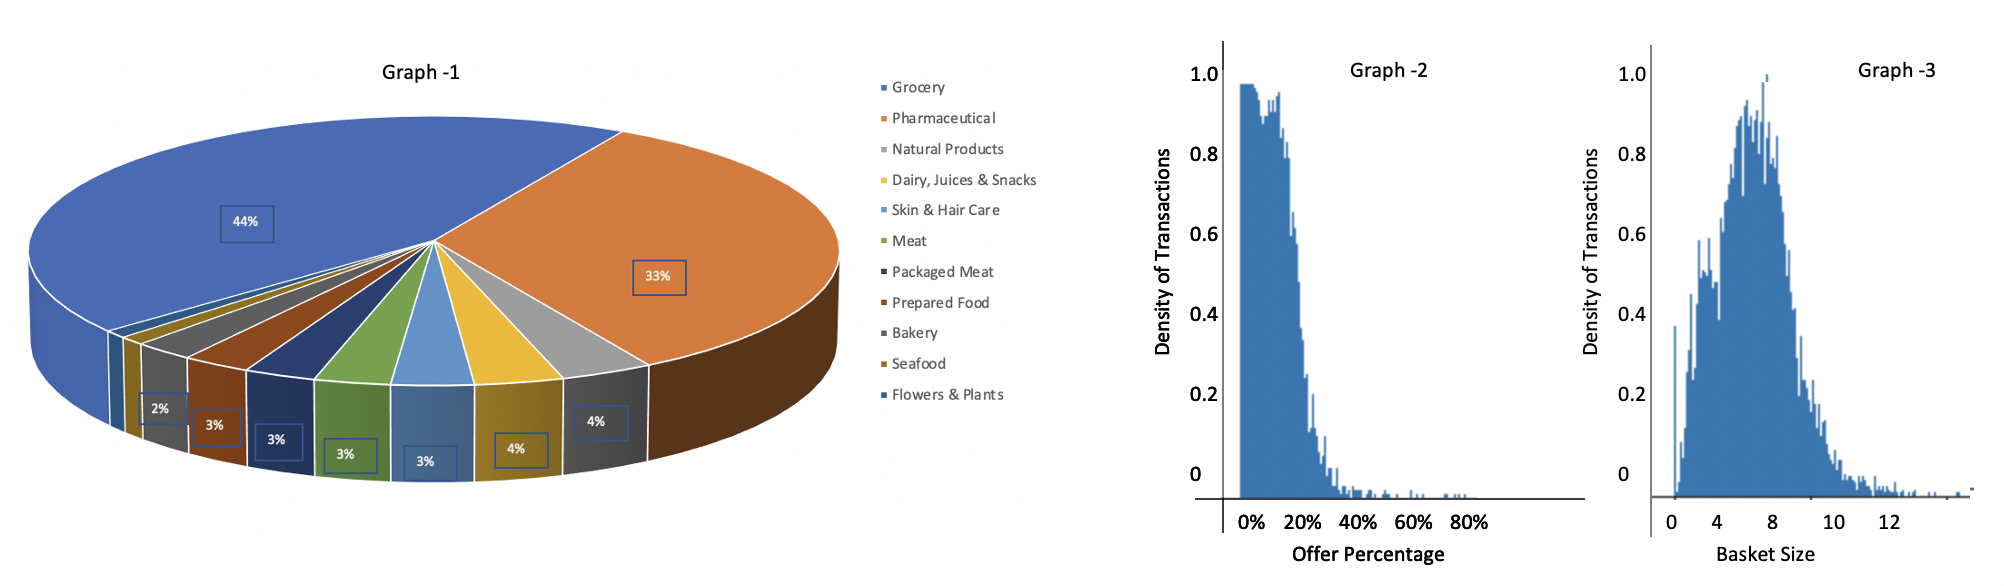
\includegraphics[width=5.5in]{img/sales_dist.png} 
    \label{fig:sales_dist} 
  \end{figure}

  \begin{figure}[t]
    \centering 
    \caption{Category graphs} 
    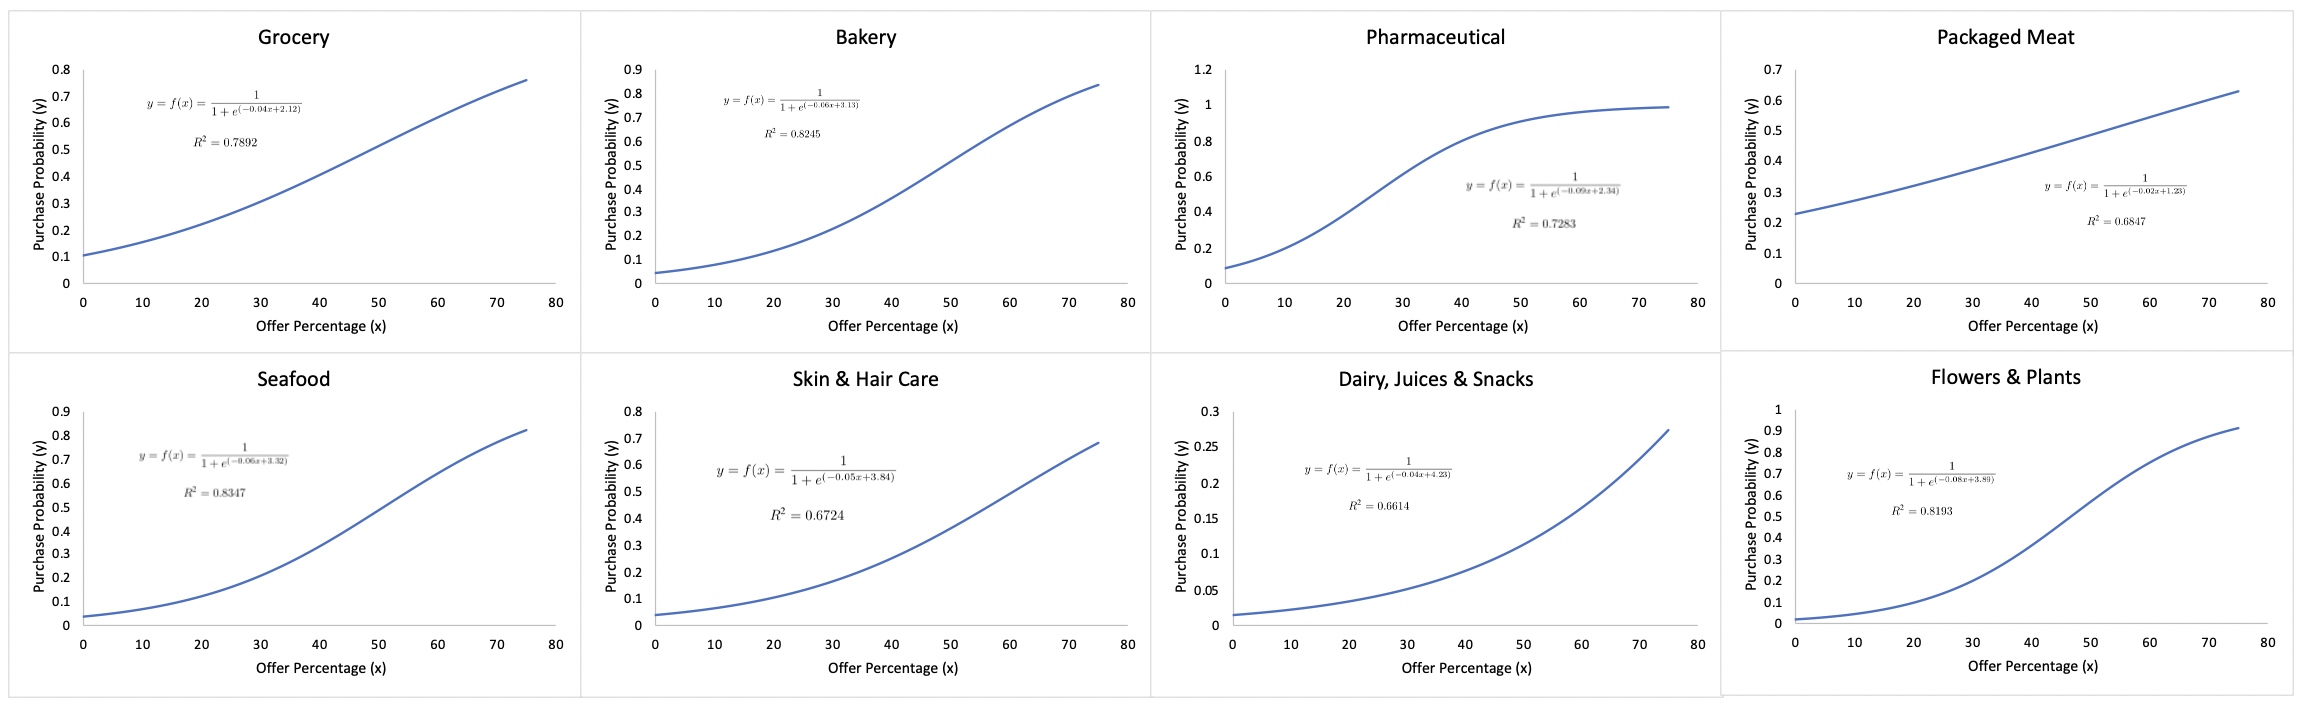
\includegraphics[width=5.5in]{img/cat_curves.png} 
    \label{fig:cat_curves} 
  \end{figure}

 \begin{figure}[t]
    \centering 
    \caption{Probability Distributions} 
    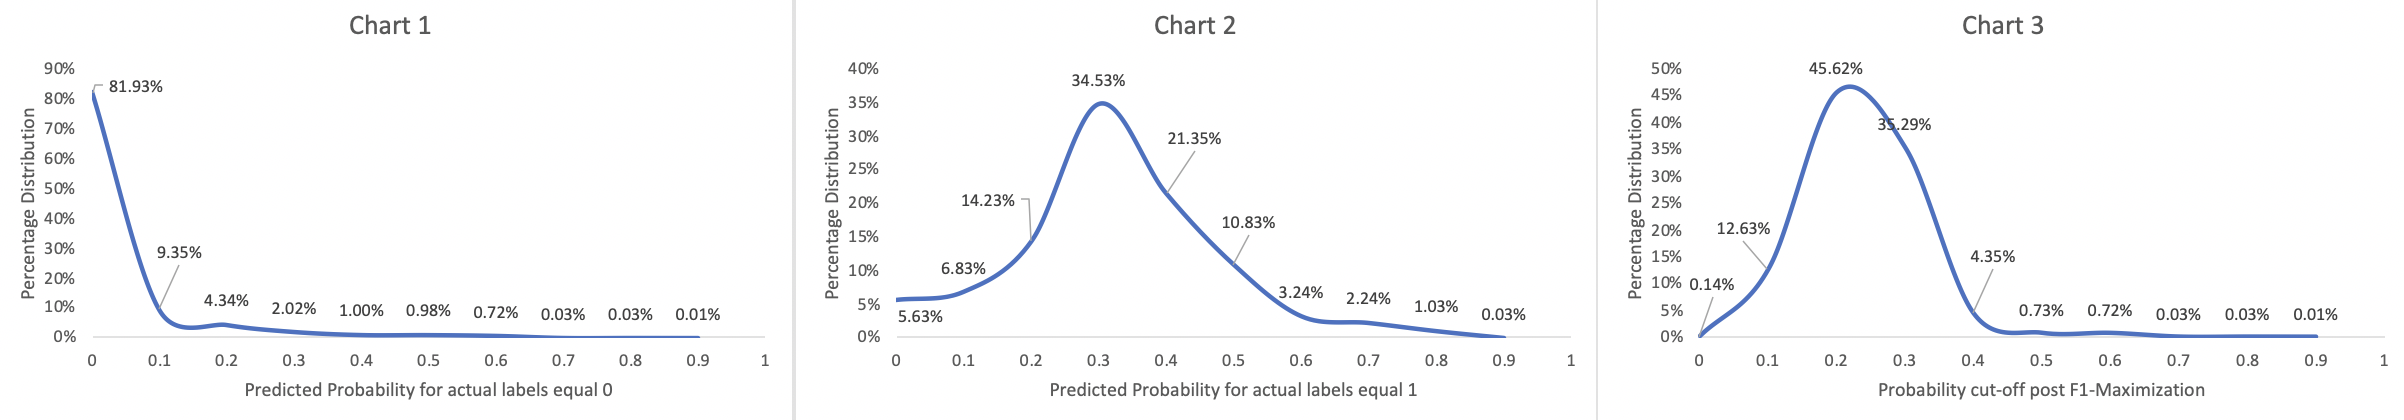
\includegraphics[width=5.5in]{img/prob_dist.png} 
    \label{fig:prob_dist} 
  \end{figure}

 \begin{figure}[t]
    \centering 
    \caption{Optimal Offers} 
    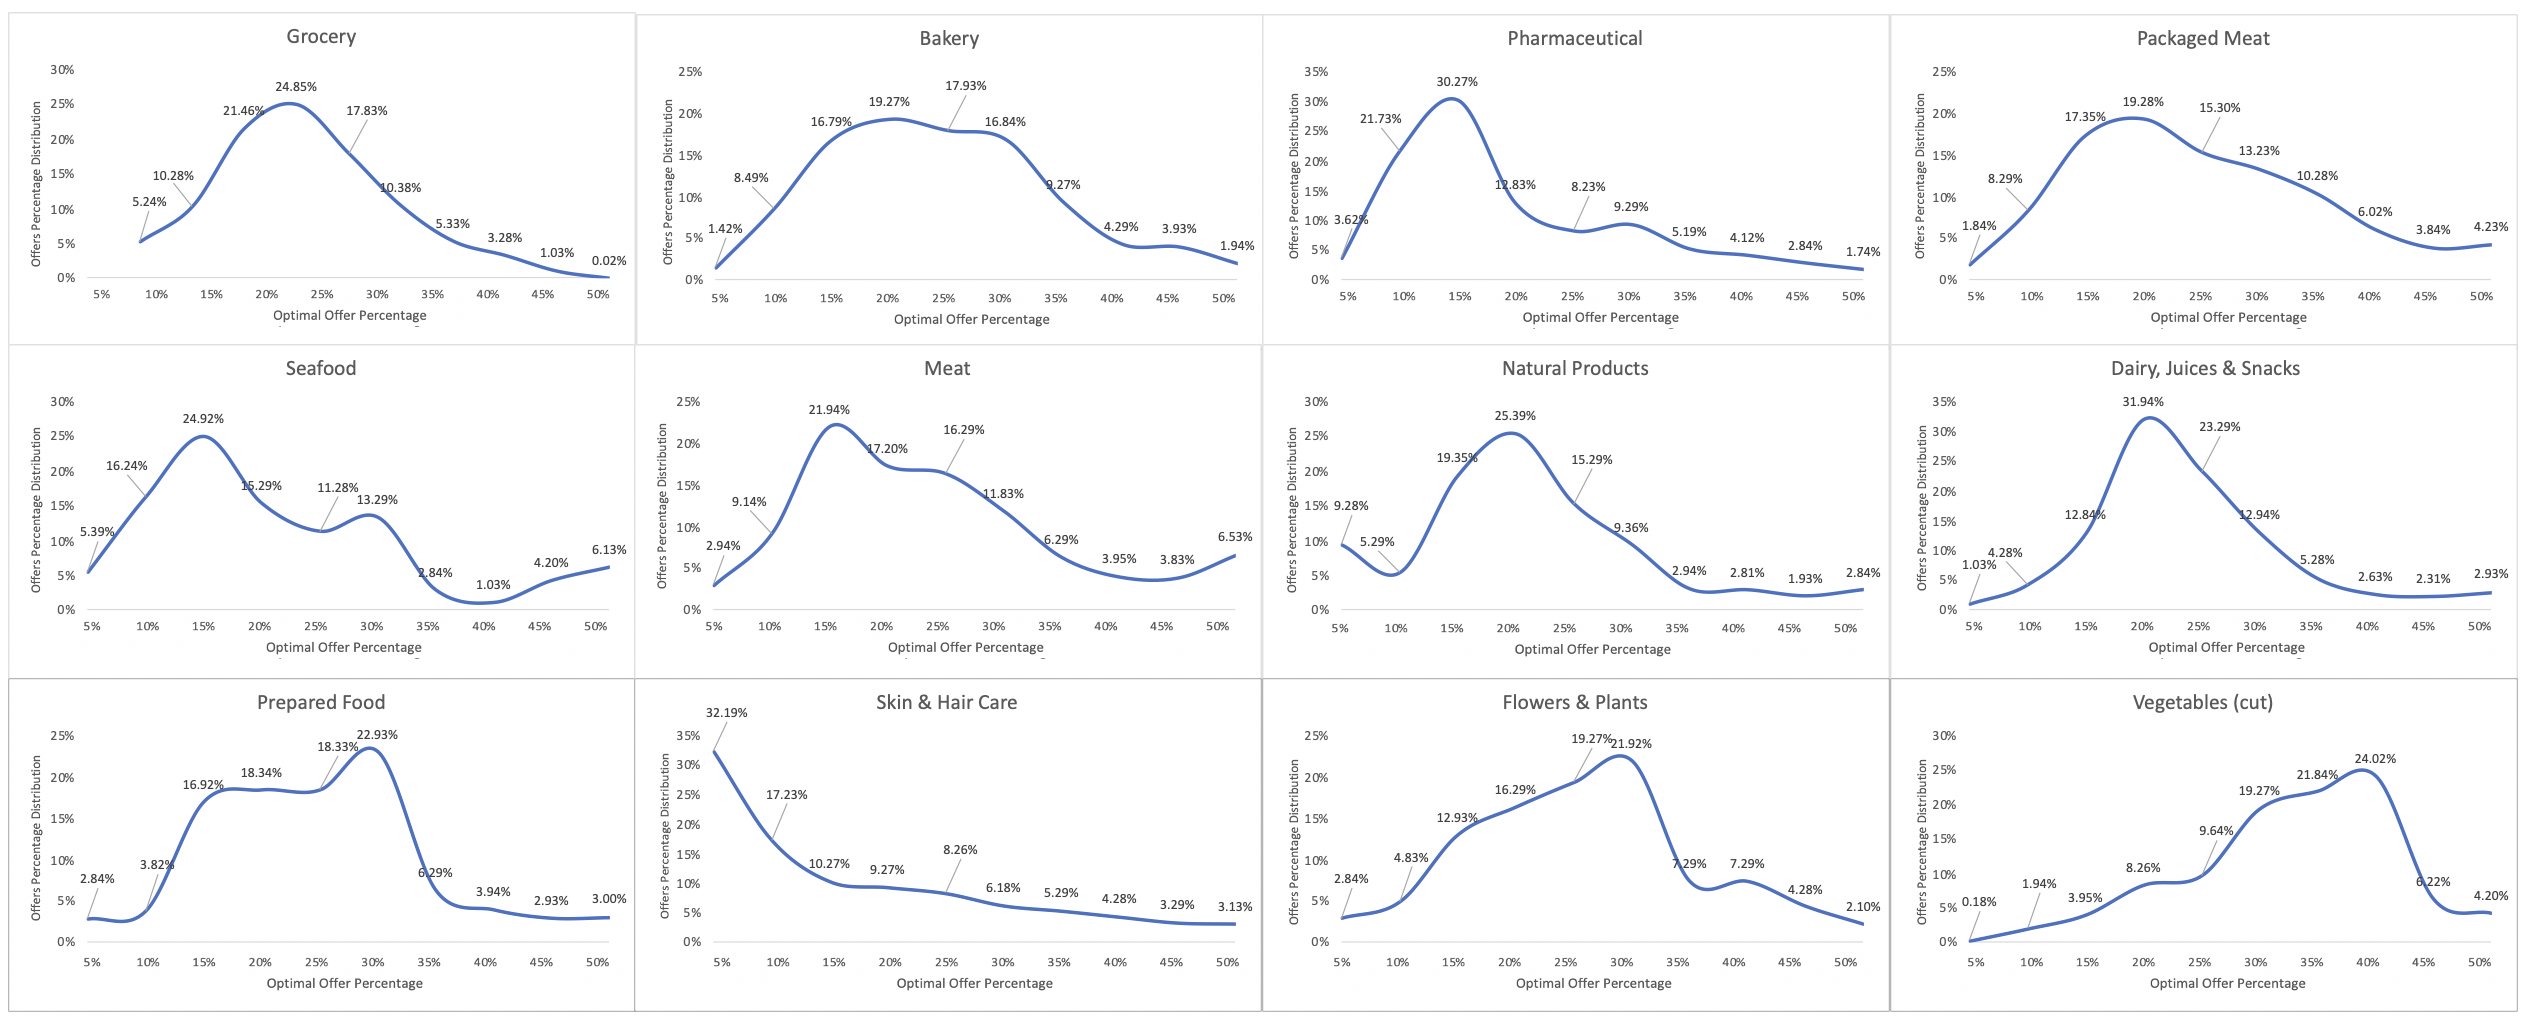
\includegraphics[width=5.5in]{img/optimize.png} 
    \label{fig:optimize} 
  \end{figure}
  
\begin{center}
\begin{table*}[!t]
\caption{Model Results and Elasticity} 
\centering
\resizebox{\textwidth}{!}{\begin{tabular}{|l|c|c|c|c|c|c|c|}
\hline
{\bf Category} & {\bf Samples} & {\bf BCELoss} & {\bf Precision} & {\bf Recall} & {\bf F\textsubscript{1}-Score} & 
{\bf Avg Elasticity} & {\bf Weighted Offer Percent} \\
\hline\hline
Grocery  		&  28,990 &  0.0283 & 0.524 & 0.501 & 0.512 & 1.13 & 23.37\\ \hline
Bakery  		&  1,628 &  0.0415 & 0.346 & 0.391 & 0.367 & 1.06 & 22.15 \\ \hline
Pharmaceutical  		&  20,492 &  0.0296 & 0.538 & 0.483 & 0.509 & 0.73 & 17.89 \\ \hline
Packaged Meat  		&  1,473 &  0.0329 & 0.473 & 0.452 & 0.462 & 0.62 & 19.15 \\ \hline
Seafood  		&  539 &  0.0382 & 0.497 & 0.379 & 0.43 & 0.89 & 16.23\\ \hline
Natural Products  		&  2,399 &  0.0319 & 0.451 & 0.524 & 0.485 & 0.95 & 21.78 \\ \hline
Dairy, Juices, Snacks  		&  2,060 & 0.0396 & 0.394 & 0.492 & 0.438 & 1.04 & 22.02\\ \hline
Prepared Food  		&  1,407 &  0.0472 & 0.338 & 0.295 & 0.315 & 1.03 & 28.27 \\ \hline
Skin, Hair Care  		&  1,906 &  0.0391 & 0.429 & 0.453 & 0.441 & 0.62 & 7.93 \\ \hline
Meat  		&  1,767 &  0.0299 & 0.498 & 0.524 & 0.511 & 0.94 & 18.92\\ \hline
Flowers, Plants  		&  491 & 0.0483 & 0.275 & 0.318 & 0.295 & 1.43 & 30.24 \\ \hline
Vegetables (cut)  		&  124 &  0.0469 & 0.364 & 0.267 & 0.308 & 1.53 & 37.92\\
\hline
\end{tabular}}
\label{tab:dlmodels}
\end{table*} 
\end{center}